\documentclass{article}
\usepackage{titling}
\usepackage{graphicx}
\usepackage{caption}
\usepackage{helvet}
\usepackage{hyperref}

\title{Relazione progetto Programmazione ad Oggetti}
\author{Alberto Canavese\\Numero matricola: 2076423}
\date{A.A. 2023/24}

\begin{document}
    % Pagina titolo
    \pretitle{\begin{center}\LARGE}
    \posttitle{\end{center}}
    \preauthor{\begin{center}\large \lineskip 0.5em}
    \postauthor{\end{center}}
    \predate{\begin{center}\large}
    \postdate{\end{center}}
    \maketitle

    % Change font to Helvetica for the rest of the document
    \renewcommand{\familydefault}{\sfdefault}

    % Pagina introduzione
    \newpage
    \section{Introduzione}
    \textbf{Sensor Hub} è un'applicazione realizzata con Qt Creator che consente di gestire tre tipi
    diversi di sensori virtuali.
    
    Il programma permette di creare, modificare, cancellare e ricercare i sensori tramite un'interfaccia
    grafica intuitiva.
        
    Vi sono due modi per dichiarare un sensore:
    \begin{itemize}
        \item \textbf{Tramite interfaccia}: Creando da zero un sensore con i dati inseriti dall'utente tramite un'opportuna finestra di dialogo.
        \item \textbf{Tramite file}: Importando, tramite finestra di dialogo, un file txt contenente i dati del sensore.
    \end{itemize} 
    La funzionalità principale di \textbf{Sensor Hub} è la possibilità di avviare una simulazione di lettura dati per un qualsiasi sensore selezionato. 
    
    La simulazione genera una serie di dati, coerenti con il tipo di sensore, che vengono visualizzati graficamente utilizzando la classe \textbf{Qt Charts}.

    Tutti i dati di simulazione e tutti i dettagli di ogni sensore vengono salvati nel medesimo file di testo, in modo da supportare la persistenza dei dati. 

    Infine, è anche possibile esportare tutti i sopracitati dati sotto forma di file \textbf{.txt} tramite un context menu, il quale permette di aprire una schermata
    di dialogo utile per selezionare il percorso di destinazione del file generato dal programma.  

    \section{Descrizione del modello}
    Il modello logico è composto da una gerarchia di classi che rappresenta i vari tipi di sensori istanziabili e simulabili. 
        
    Di seguito il diagramma UML:    
    \begin{figure}[h!]
        \centering
        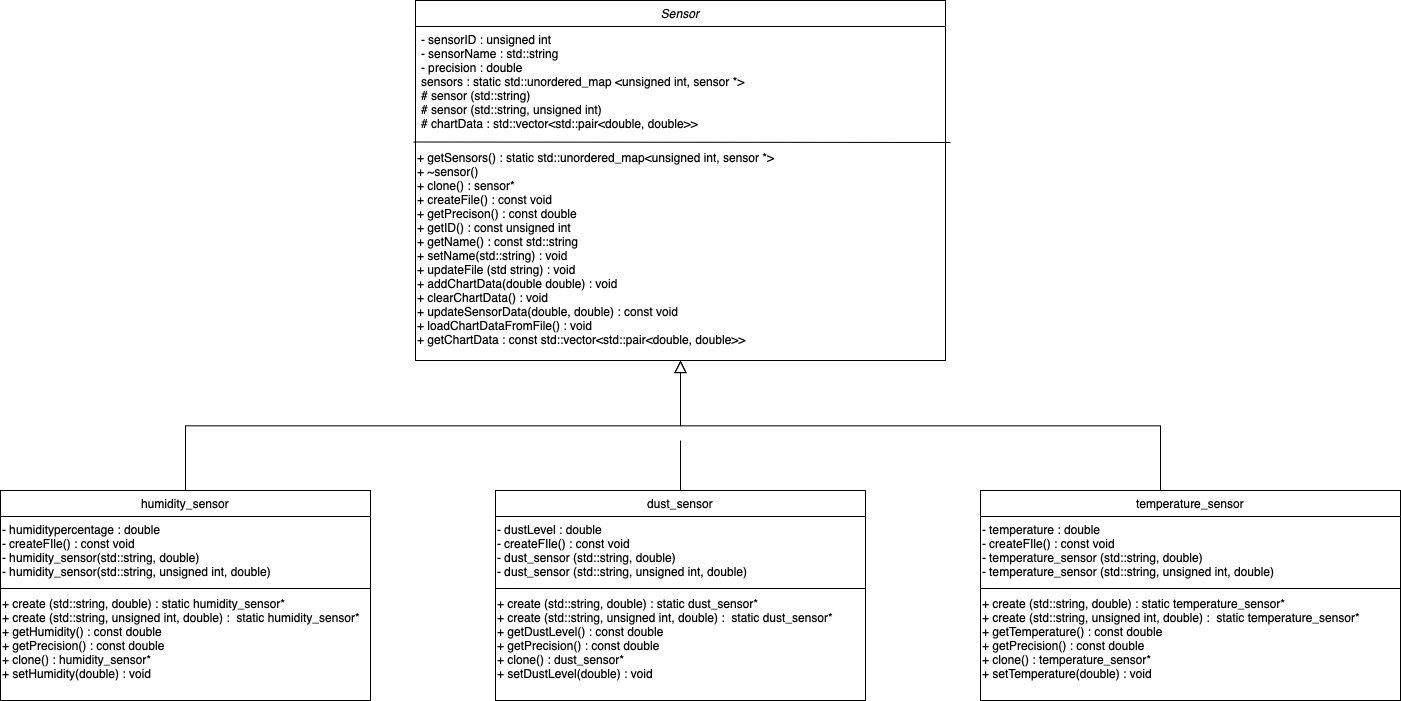
\includegraphics[width=0.8\textwidth]{UML.png}
        \caption*{Diagramma UML}
    \end{figure}
    
    \newpage
    \noindent Il modello parte da una classe astratta “sensor” che contiene le informazioni comuni a tutti i tipi di sensori, quali:
    \begin{itemize}
        \item \textbf{ID} 
        \item \textbf{Nome}
    \end{itemize} 
\end{document}
